

\section{Results}
\label{sec:results}



The postfit $m_{t\bar{t}}$ distribution of the NTMJ background, estimated using the 2D alphabet discussed in the previous section, is presented in Figure \ref{fig:mttbar_spectrum_2016} ( \ref{fig:mttbar_spectrum_20172018}) for the years 2016 (2017 and 2018), overlaid with the expected background from the $t\bar{t}$ Standard Model. The observed data are also shown. As previously published, no excess beyond the expected background is observed.

For the year 2016, since the expected limits do not exceed the previously published results (see Appendx \ref{sec:cut-based}), we remain unblinded, and the full 2016 dataset is utilized in the signal region, as illustrated in Figure~\ref{fig:mttbar_spectrum_2016}.

Subsequently, for 2017 and 2018, in principle, we could use 10\% of the data in the Pass region to remain blind, but this is not feasible, as the signal region becomes very low in statistics. Therefore, we present the fit results in the Fail region (medium not tight)



\begin{figure}[h!]
	
	\begin{center}
	     \includegraphics[width=0.49\linewidth]{Plots/2dalphabet/postfit_projy1_cen16Pass_logy.pdf} 
	     \includegraphics[width=0.49\linewidth]{Plots/2dalphabet/postfit_projy1_fwd16Pass_logy.pdf} 
		\caption{The  $t\bar{t}$ mass spectrum in the $m_{t}$ signal region (Pass) after the NTMJ background estimate using the full 2016 dataset (Unblind) for center(forward) categories left(right). }
		\label{fig:mttbar_spectrum_2016}
	\end{center}
\end{figure}

\begin{figure}[h!]
	
	\begin{center}
		\includegraphics[width=0.49\linewidth]{Plots/2dalphabet/postfit_projy1_cen17Fail_logy.pdf} 
		\includegraphics[width=0.49\linewidth]{Plots/2dalphabet/postfit_projy1_fwd17Fail_logy.pdf} \\
		
		\includegraphics[width=0.49\linewidth]{Plots/2dalphabet/postfit_projy1_cen18Fail_logy.pdf} 
		\includegraphics[width=0.49\linewidth]{Plots/2dalphabet/postfit_projy1_fwd18Fail_logy.pdf} \\
		
		\caption{Top(bottom) The  $t\bar{t}$ mass spectrum in the $m_{t}$ signal region (Fail)  after the NTMJ background estimate using the full 2017(2018) dataset for center(forward) categories left(right). }
		\label{fig:mttbar_spectrum_20172018}
	\end{center}
\end{figure}



\subsection{Limits}


In this section we compute the expected limits on $g_{kk}$, $ Z^{'}$ and $Z_{DM}$. The Upper Limit (UL) at 95 \% Confidence Level (CL) is computed using Combine software package and  is compared with the theoretical cross-section $\sigma_{th}(m)$ at Leading Order (LO).  To exclude a given signal point, the signal strength $\mu(m)$ parameter has to satisfy  
\begin{equation}
\mu(m) = \sigma_{UL}(m) / \sigma_{th}(m) < 1
\end{equation}
    


The theoretical cross section of the $g_{kk}$ are given in table ~\ref{table:RSGluonTheoryXS} and the expected limits are shown in Figure~\ref{fig:limits_run2} with the expected mass limits shown in Table~\ref{tab:limits}.
%\begin{table}[h!]
%	\centering
%	
%	\begin{tabular}{| c c |}\hline
%			\multicolumn{2}{| c |}{\textbf{ $g_{KK}$ }} \\ \hline
%			 \textbf{Mass TeV} & \textbf{$ \sigma $ (pb)} \\ \hline
%		\hline
%		
%		1.0 & 20.05 \\
%		1.5 & 3.519 \\
%		2.0 & 0.9528 \\
%		2.5 & 0.3136 \\
%		3.0 & 0.1289 \\
%		3.5 & 0.0545 \\
%		4.0 & 0.02807 \\
%		4.5 & 0.01603 \\
%		5.0 & 0.009095 \\
%		
%		\hline
%	\end{tabular}
%	
%	\caption{Expected (theory) cross sections for $g_{kk}$ gluon signal mass points}
%	\label{table:RSGluonTheoryXS}
%\end{table}

\newcommand{\ColTitle}[1]{\multicolumn{2}{|P{4cm}|}{\bf #1}} % For use in table below
\newcommand{\ColMass}{\multicolumn{1}{|P{2cm}|}{\bf Mass $(TeV)$}}
\newcommand{\ColXS}{\multicolumn{1}{|P{2cm}|}{\bf$\sigma\ (pb)$}}


\begin{figure}[!htbp]
	\begin{center}
		\includegraphics[width=0.49\linewidth]{Plots/results/limits_combine_rsgluon_all_0424.pdf} 
		\includegraphics[width=0.49\linewidth]{Plots/results/limits_combine_zprime1_all_0424.pdf} \\ 
		\includegraphics[width=0.49\linewidth]{Plots/results/limits_combine_zprime10_all_0424.pdf} 
		\includegraphics[width=0.49\linewidth]{Plots/results/limits_combine_zprime30_all_0424.pdf} \\
		\includegraphics[width=0.49\linewidth]{Plots/results/limits_combine_zprimedm_all_0424.pdf} 


		\caption{ The expected Run 2 limits for $g_{kk}$ mass for (top left), $Z'$ mass  with 1 \% width (top right),  $Z'$ mass  with 10 \% width (middle left),  $Z'$ mass  with 30 \% width (middle right), and  Run 2 (bottom)}
		\label{fig:limits_run2}
	\end{center}
\end{figure}


\begin{table}[h]
\centering
\begin{tabular}{|c|c|}
\hline
\textbf{Signal} & \textbf{Mass [TeV]} \\ \hline
$g_{kk}$ & $4.45 \pm 0.03$ \\
$Z'$ 1\% width & $3.93 \pm 0.01$ \\
$Z'$ 10\% width & $5.20 \pm 0.02$ \\
$Z'$ 30\% width & $6.62 \pm 0.04$ \\
$Z'_{DM}$ & $3.31 \pm 0.01$ \\ \hline 
\end{tabular}
\caption{Expected Run 2 mass limits.}
\label{tab:limits}
\end{table}

% {'zprimeDM_high': [3.3076, 0.005738549625000002], 'zprime1': [3.9280999999999997, 0.0034085711910000014], 'zprimeDM': [1.4472, 0.5678441562499985], 'zprime30': [6.6171999999999995, 0.030261901290000007], 'rsgluon': [4.4510000000000005, 0.022389491999999993], 'zprime10': [5.198799999999999, 0.012516775194499999]}

\newcolumntype{P}[1]{>{\centering\arraybackslash}p{#1}}



%\begin{table}[h!]
%  \begin{center}
%  \begin{tabular}{|P{2cm}P{2cm}|P{2cm}P{2cm}|P{2cm}P{2cm}|}\hline
%    \ColTitle{$Z'\ 10\%$ Width} & \ColTitle{$Z'\ 30\%$ Width} & \ColTitle{$Z'$ DM}\\ \hline
%    \ColMass & \ColXS & \ColMass & \ColXS & \ColMass & \ColXS \\ \hline
%    1.0 & 44.8526 & 1.0 & 129.361 & 1.0 & 2.222 \\ 
%    1.5 & -- & 1.5 & -- & 1.5 & 0.387 \\ 
%    2.0 & 2.26215 & 2.0 & 7.74166 & 2.0 &  0.09428 \\ 
%    2.5 & 0.734314 & 2.5 & 2.79430 & 2.5 & 0.0279  \\ 
%    3.0 & 0.272788 & 3.0 & 1.17252 & 3.0 & 0.009327  \\ 
%    3.5 & 0.112874 & 3.5 & 0.553916 & 3.5 & 0.003507  \\ 
%    4.0 & 0.0515542 & 4.0 & 0.0288839 & 4.0 & 0.001484 \\ 
%    4.5 & 0.0259114 & 4.5 & 0.163747 & 4.5 & 0.0007087, \\ 
%    5.0 & 0.0142839 & 5.0 & 0.0995997 & 5.0 & -0.0003801\\
%            
%    \hline
%  \end{tabular}
%  \caption{Expected (theory) cross sections for the corresponding $Z'$ signal mass points}
%  \label{table:ZprimeTheoryXS}
%  \end{center}
%\end{table}

\begin{table}[h!]
  \begin{center}
  \begin{tabular}{|P{2cm}P{2cm}|P{2cm}P{2cm}|}\hline
    \ColTitle{$g_{KK}$} & \ColTitle{$Z'$ DM} 		\\ \hline
    \ColMass & \ColXS & \ColMass & \ColXS  		\\ \hline
    1.0 & 20.05 		& 1.0 & 0.3637				\\ 
    1.5 & 3.519 		& 1.5 & 0.1821				\\
    2.0 & 0.9528		& 2.0 & 0.01886			\\ 
    2.5 & 0.3136 	& 2.5 & 0.005887			\\ 
    3.0 & 0.1289 	& 3.0 & 0.002111			\\ 
    3.5 & 0.0545 	& 3.5 & 8.559$\times10^{-4}$	\\ 
    4.0 & 0.02807 	& 4.0 & 3.873$\times10^{-4}$	\\ 
    4.5 & 0.01603 	& 4.5 & 1.969$\times10^{-4}$	\\ 
    5.0 & 0.009095	& 5.0 & 1.082$\times10^{-4}$	\\
     
    \hline
  \end{tabular}
  \caption{Expected (theory) cross sections for $g_{kk}$ and $Z'_{DM}$ signal mass points~\cite{CMS:xsdb}.}
  \label{table:RSGluonTheoryXS}
  \end{center}
\end{table}

\begin{table}[h!]
  \begin{center}
  \begin{tabular}{|P{2cm}P{2cm}|P{2cm}P{2cm}|P{2cm}P{2cm}|}\hline
    \ColTitle{$Z'\ 1\%$ Width} & \ColTitle{$Z'\ 10\%$ Width} & \ColTitle{$Z'\ 30\%$ Width}\\ \hline
    \ColMass & \ColXS & \ColMass & \ColXS & \ColMass & \ColXS \\ \hline
    1.0 & 3.532  		& 1.0 & 0.3637			& 1.0 & 0.1085			\\ 
    1.2 & 1.735			& 1.2 & 0.1821			& 1.2 & 0.05567			\\
    1.4 & 0.9136		& 1.4 & 0.09676			& 1.4 & 0.03084			\\
    1.6 & 0.4943		& 1.6 & 0.05402			& 1.6 & 0.01773			\\ 
    1.8 & 0.2848		& 1.8 & 0.03152			& 1.8 & 0.01072			\\ 
    2.0 & 0.1656		& 2.0 & 0.01886			& 2.0 & 0.006683		\\ 
    2.5 & 0.04757.      & 2.5 & 0.005887		& 2.5 & 0.002336		\\ 
    3.0 & 0.01477	& 3.0 & 0.002111		& 3.0 & 9.484$\times10^{-4}$	\\ 
    3.5 & 0.005054	& 3.5 & 8.559$\times10^{-4}$	& 3.5 & 8.559$\times10^{-4}$	\\ 
    4.0 & 0.00189	& 4.0 & 3.873$\times10^{-4}$	& 4.0 & 3.873$\times10^{-4}$	\\ 
    4.5 & 0.0007732	& 4.5 & 1.969$\times10^{-4}$	& 4.5 & 1.969$\times10^{-4}$	\\ 
    5.0 & 3.217$\times10^{-5}$	& 5.0 & 1.082$\times10^{-4}$	& 5.0 & 1.082$\times10^{-4}$	\\
    6.0 & 6.06$\times10^{-5}$	& 6.0 & 4.159$\times10^{-5}$	& 6.0 & 3.302$\times10^{-5}$	\\
    7.0 & 1.154$\times10^{-5}$	& 7.0 & 1.933$\times10^{-5}$	& 7.0 & 1.676$\times10^{-5}$	\\

     
    \hline
  \end{tabular}
  \caption{Expected (theory) cross sections for the corresponding $Z'$ signal mass points~\cite{NLOtheoryCurves}.}
  \label{table:ZprimeTheoryXS}
  \end{center}
\end{table}


\clearpage

\subsection{Impact}

The significance of a nuisance parameter (NP) is determined by measuring its impact and pull.   The difference between the best fit value of the NP to its pre-fit value defines the pull and is defined in following : 
\begin{equation}
	\mathrm{pull} = \frac{\hat{\theta}-\theta}{\sigma_\theta}\,,
\end{equation}
where \(\hat{\theta}\) is the best-fit value of the NP, \(\theta\) is the initial (pre-fit) value, conventionally set to zero, and \(\sigma_\theta\) is the input uncertainty. Meanwhile, the impact of an NP on a parameter of interest (POI) is the shift in the best-fit value of the POI when the NP is fixed to $\pm 1 \sigma$ of its nominal value. A low impact indicates that the NP has a negligible effect on the POI. 

\begin{equation}
	\mathrm{impact} = \Delta \mu^{\pm}=\hat{\hat{\mu}}_{\theta \pm \sigma_{\theta}}-\hat{\mu}\,.
\end{equation}

An impact plot, as shown in Figure \ref{fig:impacts}, displays the impacts of the NPs on the POIs. The highest impacts on the results come from fit NPs, as well as the $t\bar{t}$ xsec and $q^{2}$ uncertainties.

\begin{figure}[!htbp]
	\begin{center}
		\includegraphics[width=1.0\linewidth]{Plots/results/impacts_nobins.pdf} 
		\caption{Blinded Impacts for Run 2 data taking ranked in decreasing significance.}
		\label{fig:impacts}
	\end{center}
\end{figure}

\clearpage


\clearpage


\section{Statistical Analysis}
\label{sec:stats}

In this section, the obtained NTMJ background yields from the background estimation method in the signal region are presented, and the statistical evaluation used to exclude specific signal scenarios is discussed.


\subsection{F-Tests}
\label{sec:ftests}

F-tests were performed to evaluate the best transfer function for each year and rapidity region. The F-Test compares the likelihood ratios of a higher order transfer function to a lower order transfer function. The test statistic for the F-test is

\begin{equation}
	F = \frac{ -2 \ln{(\lambda_1)(\lambda_2)}/(p_2 - p_1)}{-2 \ln{(\lambda_2)}(n - p_2)}	
\end{equation}}

where $\lambda_1$ ($\lambda_2$) is the likelihood ratio of the lower (higher) order transfer function, $p_1$ ($p_2$) is the number of parameters in the lower (higher) order transfer function, and $n$ is the number of degrees of freedom.

The linear transfer functions (1x0 and 0x0) are first compared to the constant 0x0 transfer function. The 1x1 transfer function is then compared to the 0x1 and 1x0 functions. If the p-value is low (p-value < 0.3), then the 1x1 function is chosen. Higher order transfer functions are also compared to 1x1. In some cases the 2x1 is better according to the FTest, but the uncertainties on the parameters are very large. For all years, the 1x1 function is used for the forward regions, and the 0x1 for the central regions, as listed in Table~\ref{tab:TF}. The plots of the distributions of the F-Test statistic are shown in Appendix~\ref{sec:appendix_ftests}. The transfer function comparison which yields the lowest p-value is chosen for the background estimate. The functions tested are:

$$ 0x0 = a $$
$$ 1x0 = a + b_1 m_t $$
$$ 0x1 = a + b_1 m_{t\bar{t}} $$
$$ 1x1 = (a + b_1 m_t)( 1 + c_1 m_{t\bar{t}}) $$
$$ 2x1 = (a + b_1 m_t + b_2 m_t^2)( 1 + c_1 m_{t\bar{t}}) $$
$$ 1x2 = (a + b_1 m_t)( 1 + c_1 m_{t\bar{t}} + c_2 m_{t\bar{t}}^2) $$



\begin{table}[h!]
\centering
\begin{tabular}{|| c c c ||} 
 \hline
 Year & central TF  & forward TF  \\
 \hline\hline
 2016 & 0x1 & 1x1  \\ 
 2017 & 0x1 & 1x1  \\ 
 2018 & 0x1 & 1x1  \\ 
 \hline
\end{tabular}
\caption{Transfer functions selected for each year and rapidity region.}
\label{tab:TF}
\end{table}

\clearpage


\clearpage




\subsection{Goodness of Fit}
\label{sec:gof}


We perform a goodness of fit test for each of the 6 fits. The test statistic $q$ is 

$$ q = -2 \ln \lambda $$

where $\lambda$ is the ratio of the likelihoods of the model to the saturated model.

The results of the goodness of fit tests for Run 2 is shown in Figure~\ref{fig:gof_run2}. The Goodness of Fit run separately for all years and rapidity regions yield a p-value > 0.1, and are shown in Appendix~\ref{sec:appendix_gof}.

           
\begin{figure}[!htbp]
                \begin{center}
                 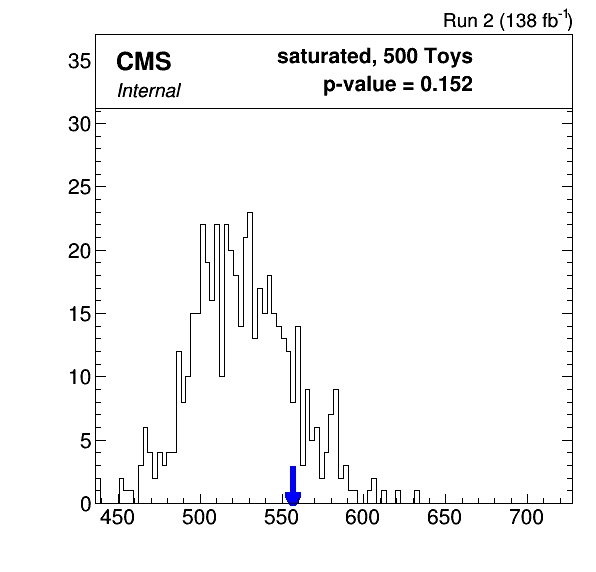
\includegraphics[width=0.5\linewidth]{Plots/tests/gof_plot_run2.pdf}

                    \caption{Goodness of Fit test for combined Run 2.}
                    \label{fig:gof_run2}
                \end{center}
            \end{figure}          
            
            
\subsection{Signal Injection}
\label{sec:siginj}

We perform a signal injection test to evaluate the tendency of the fit to model the signal contribution to data. To do this, we generate 100 toy models with a known signal contribution ($r_{inj} = 0$ for background only and $r_{inj} = 1$ for background+signal), then fit the model and compare the fitted $r$ to the known $r_{inj}$ in a pull plot using Equation~\ref{eq:si}. The signal injection tests conclude that the models for each year and rapidity region neither over-model nor under-model the signal contribution.

\begin{equation}
	P = \frac{r - r_{inj}}{r_{err}}
\label{eq:si}
\end{equation} 

The results of the signal injection tests are shown in Figures~\ref{fig:si16}~-~\ref{fig:si18}.


	\begin{figure}[!htbp]
                \begin{center}
                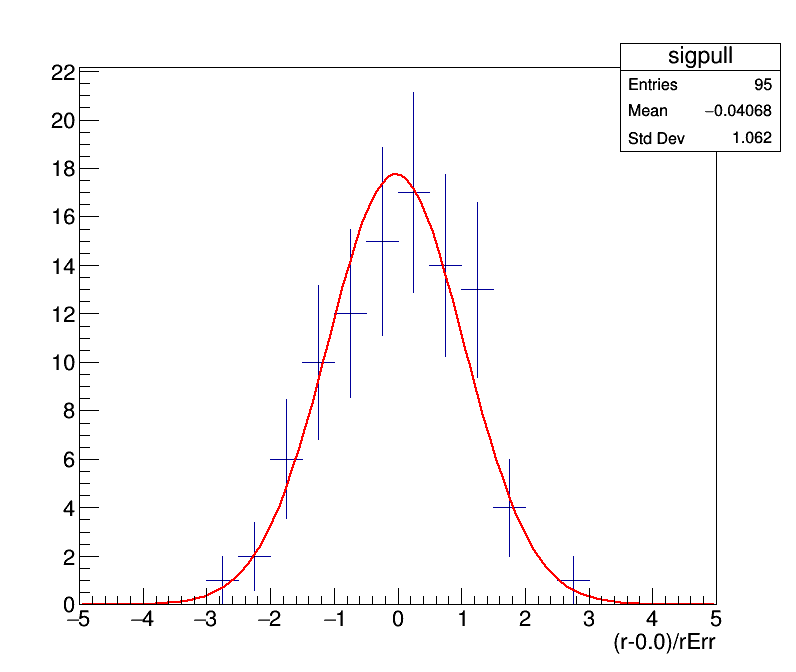
\includegraphics[width=0.45\linewidth]{Plots/tests/signalInjection_r0p0_pull_cen16.png}
                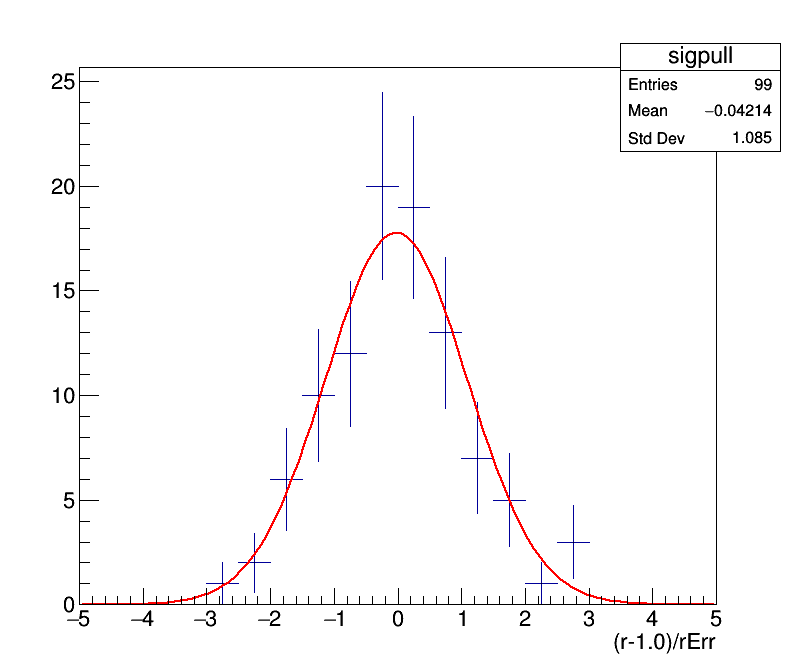
\includegraphics[width=0.45\linewidth]{Plots/tests/signalInjection_r1p0_pull_cen16.png} \\
                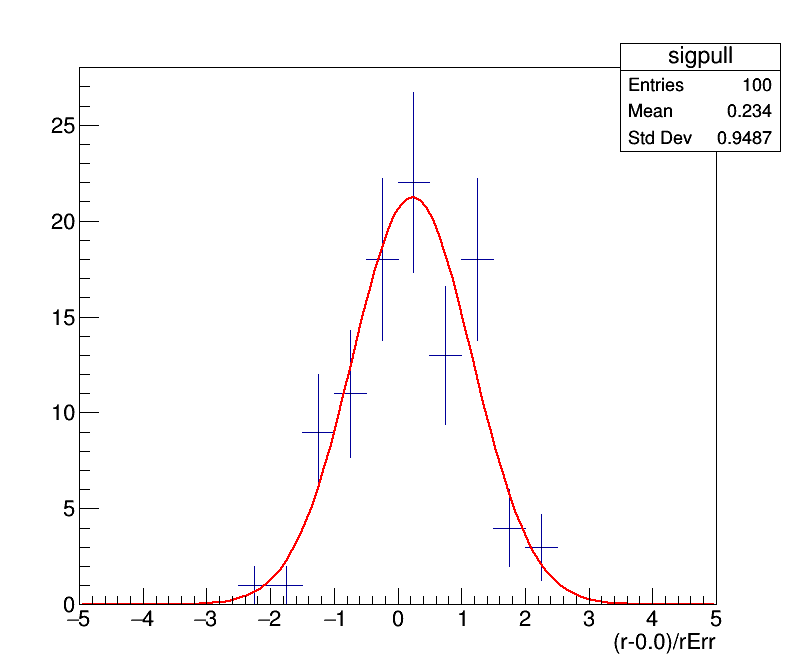
\includegraphics[width=0.45\linewidth]{Plots/tests/signalInjection_r0p0_pull_fwd16.png}
                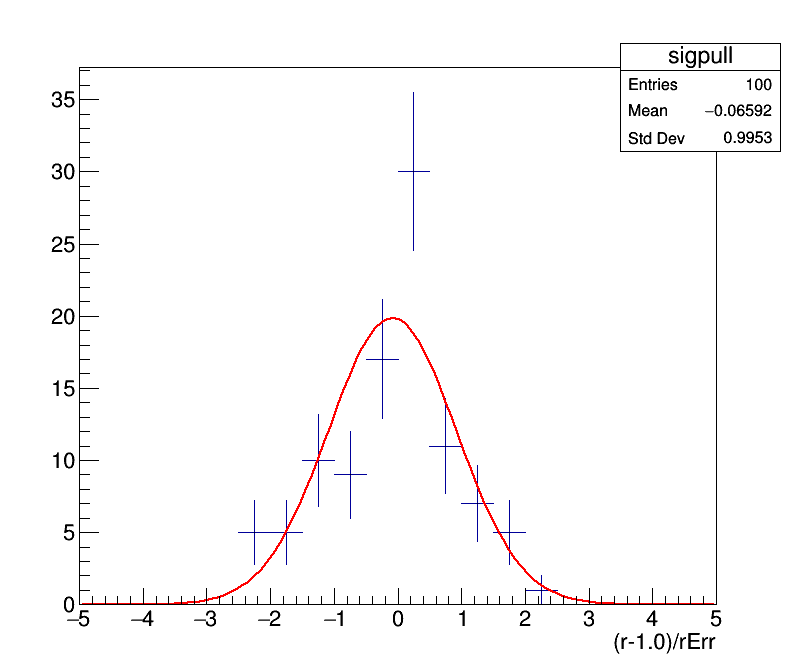
\includegraphics[width=0.45\linewidth]{Plots/tests/signalInjection_r1p0_pull_fwd16.png} \\
    
                    \caption{Signal Injection test for 2016 central (top) and forward (bottom), with $r_{inj} = 0$ (left) and $r_{inj} = 1$ (right).}
                    \label{fig:si16}
                \end{center}
            \end{figure}
            
          \begin{figure}[!htbp]
                \begin{center}
                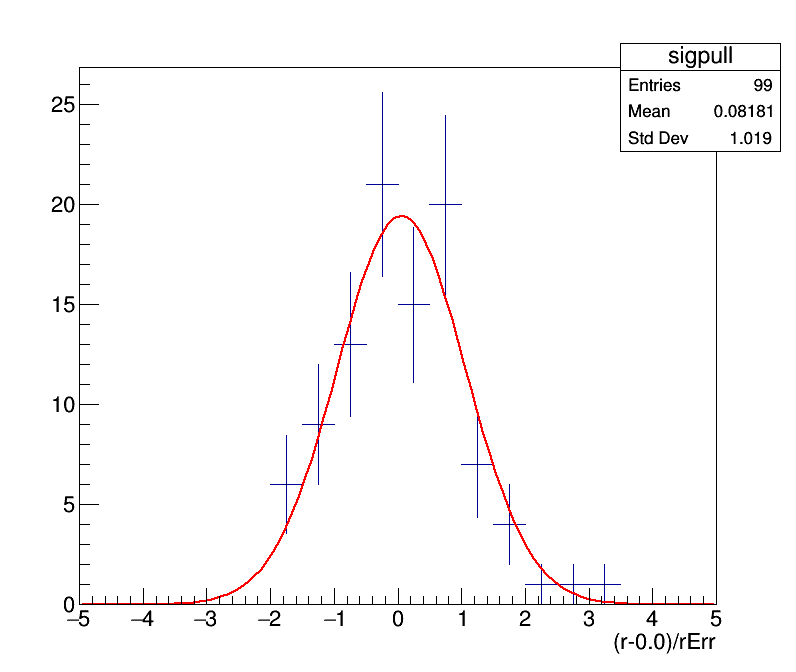
\includegraphics[width=0.45\linewidth]{Plots/tests/signalInjection_r0p0_pull_cen17.png}
                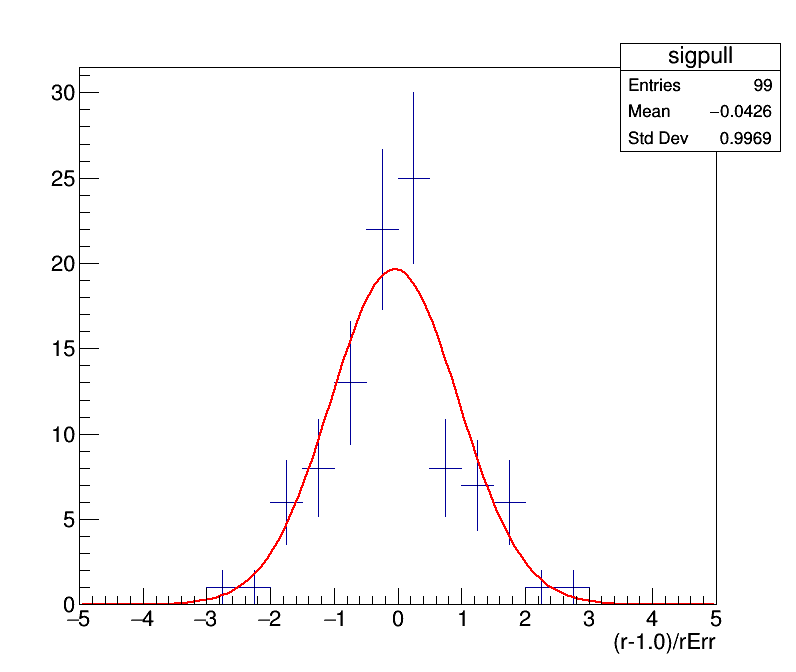
\includegraphics[width=0.45\linewidth]{Plots/tests/signalInjection_r1p0_pull_cen17.png} \\
                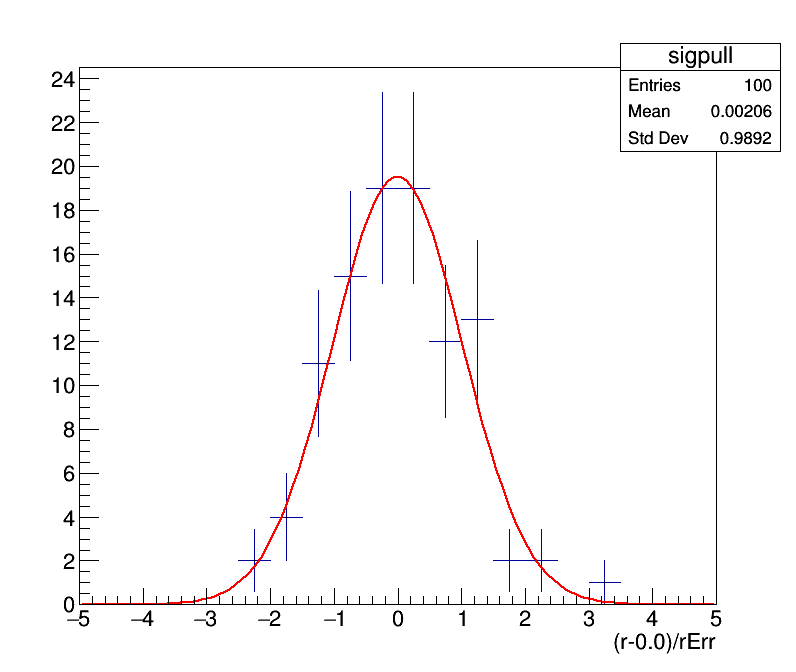
\includegraphics[width=0.45\linewidth]{Plots/tests/signalInjection_r0p0_pull_fwd17.png}
                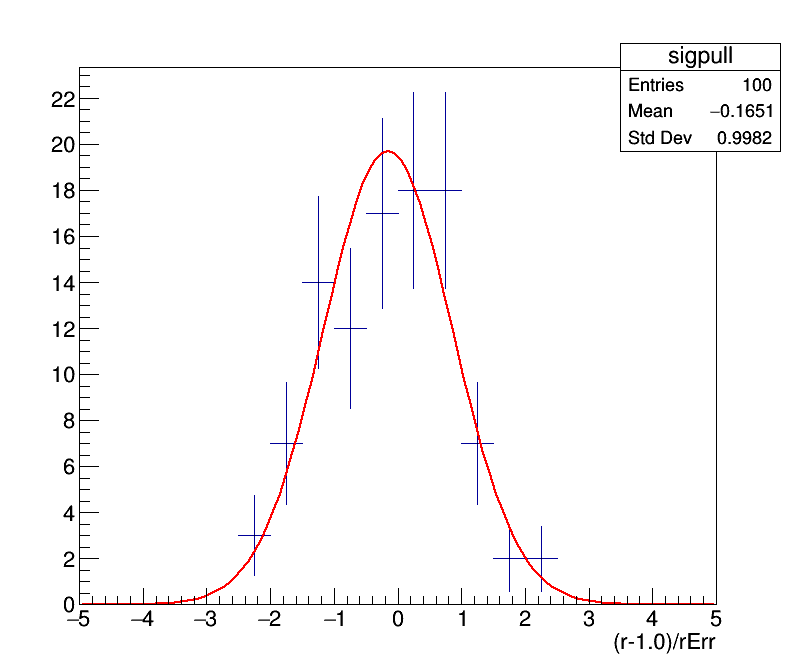
\includegraphics[width=0.45\linewidth]{Plots/tests/signalInjection_r1p0_pull_fwd17.png} \\
    
                    \caption{Signal Injection test for 2017 central (top) and forward (bottom), with $r_{inj} = 0$ (left) and $r_{inj} = 1$ (right).}
                    \label{fig:si17}
                \end{center}
            \end{figure}
            
          \begin{figure}[!htbp]
                \begin{center}
                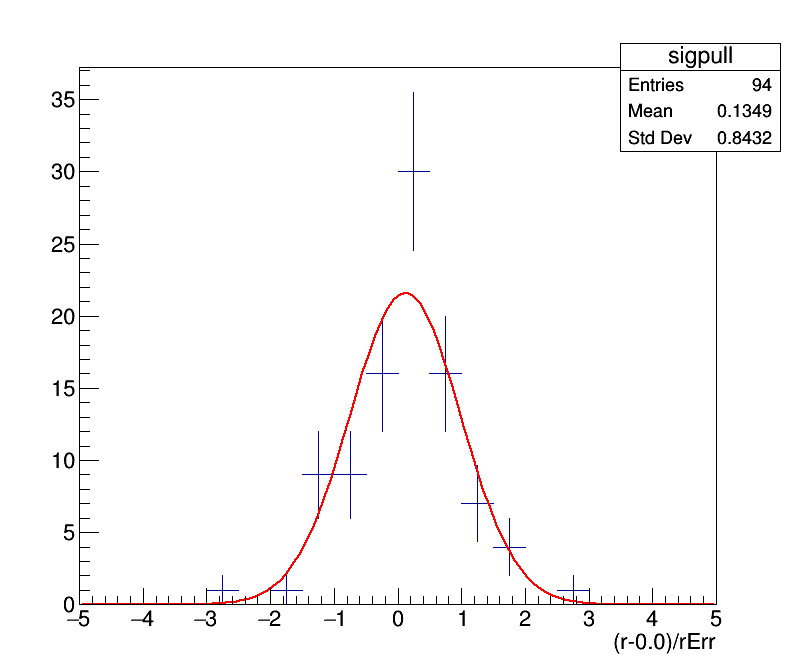
\includegraphics[width=0.45\linewidth]{Plots/tests/signalInjection_r0p0_pull_cen18.png}
                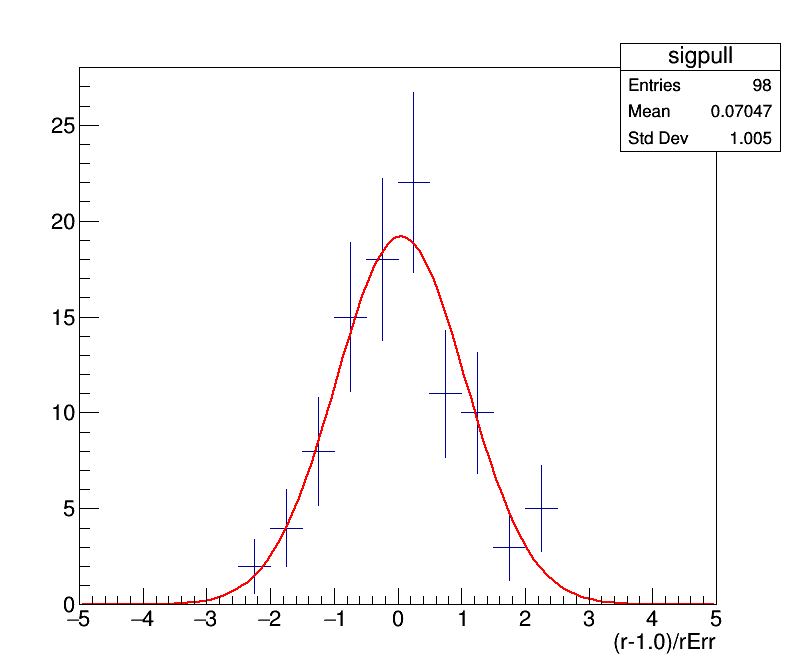
\includegraphics[width=0.45\linewidth]{Plots/tests/signalInjection_r1p0_pull_cen18.png} \\
                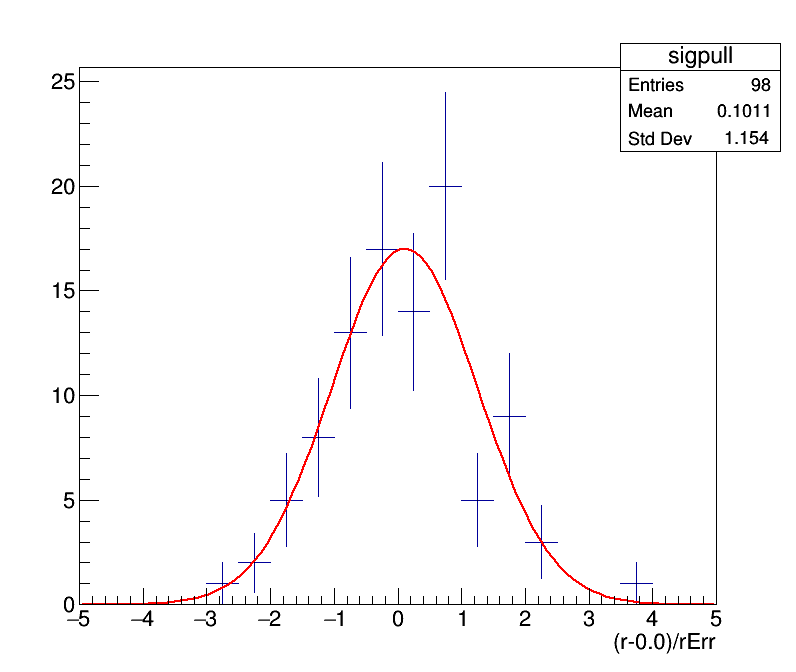
\includegraphics[width=0.45\linewidth]{Plots/tests/signalInjection_r0p0_pull_fwd18.png}
                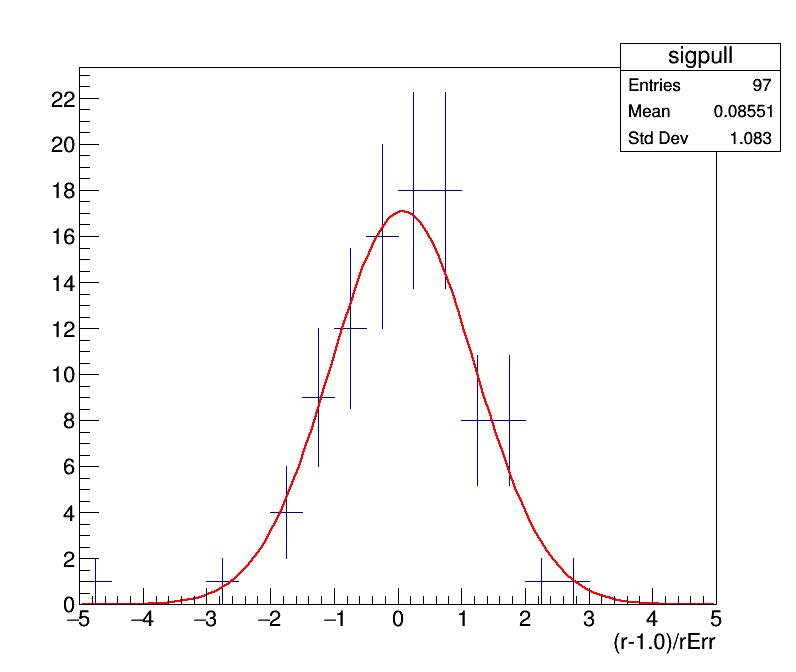
\includegraphics[width=0.45\linewidth]{Plots/tests/signalInjection_r1p0_pull_fwd18.png} \\
    
                    \caption{Signal Injection test for 2018 central (top) and forward (bottom), with $r_{inj} = 0$ (left) and $r_{inj} = 1$ (right).}
                    \label{fig:si18}
                \end{center}
            \end{figure}
            
            
            
            
\clearpage

